
\begin{figure}
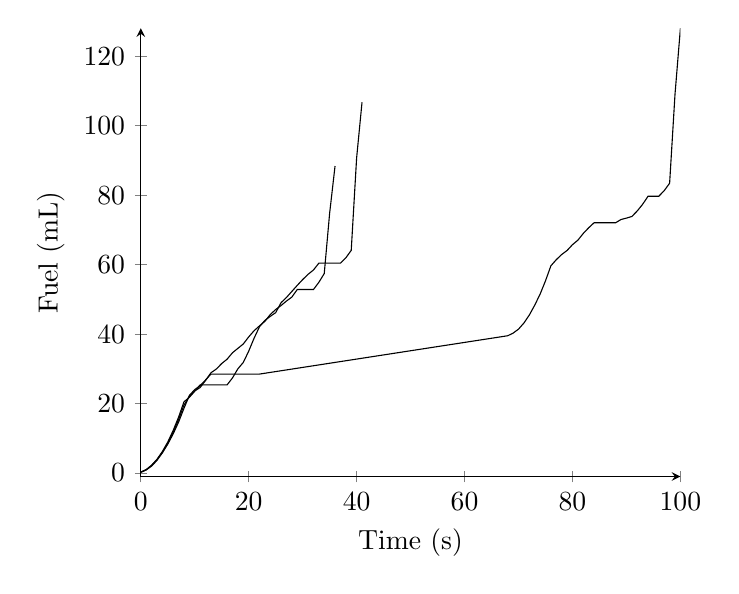
\begin{tikzpicture}
\begin{axis}[
legend style={anchor=west},
axis x line=bottom,
axis y line=left,
ymin=-1,
xlabel=Time (s),
ylabel=Fuel (mL),
]
\addplot[] coordinates {
(0, 0.239885513361)
(1, 0.936108937325)
(2, 2.23258215438)
(3, 3.95006742508)
(4, 6.20522829578)
(5, 8.91579058584)
(6, 12.253650053)
(7, 16.0583593021)
(8, 20.4966706882)
(9, 21.8045822088)
(10, 23.5683807651)
(11, 25.3894632718)
(12, 25.3894632718)
(13, 25.3894632718)
(14, 25.3894632718)
(15, 25.3894632718)
(16, 25.3894632718)
(17, 27.4003585656)
(18, 30.0215816561)
(19, 31.85292494)
(20, 35.0941613642)
(21, 38.8218521669)
(22, 42.1235075444)
(23, 43.9430939168)
(24, 45.1147392633)
(25, 46.1839118445)
(26, 49.0561683266)
(27, 50.5497568756)
(28, 52.2940165189)
(29, 54.0359565286)
(30, 55.7001126205)
(31, 57.208650749)
(32, 58.4549704422)
(33, 60.4227885081)
(34, 60.4227885081)
(35, 60.4227885081)
(36, 60.4227885081)
(37, 60.4227885081)
(38, 61.9571846562)
(39, 64.1037376146)
(40, 90.7315038937)
(41, 106.733639799)
};
\addplot[] coordinates {
(0, 0.239885513361)
(1, 0.985574203373)
(2, 2.19728620842)
(3, 3.79125666634)
(4, 5.87931838914)
(5, 8.33055472232)
(6, 11.2587271265)
(7, 14.6473805468)
(8, 18.6142354257)
(9, 22.3381459645)
(10, 24.0344591938)
(11, 25.1579629202)
(12, 26.7858466181)
(13, 28.4956707955)
(14, 28.4956707955)
(15, 28.4956707955)
(16, 28.4956707955)
(17, 28.4956707955)
(18, 28.4956707955)
(19, 28.4956707955)
(20, 28.4956707955)
(21, 28.4956707955)
(22, 28.4956707955)
(23, 28.7355563088)
(24, 28.9754418222)
(25, 29.2153273356)
(26, 29.4552128489)
(27, 29.6950983623)
(28, 29.9349838756)
(29, 30.174869389)
(30, 30.4147549024)
(31, 30.6546404157)
(32, 30.8945259291)
(33, 31.1344114424)
(34, 31.3742969558)
(35, 31.6141824692)
(36, 31.8540679825)
(37, 32.0939534959)
(38, 32.3338390093)
(39, 32.5737245226)
(40, 32.813610036)
(41, 33.0534955493)
(42, 33.2933810627)
(43, 33.5332665761)
(44, 33.7731520894)
(45, 34.0130376028)
(46, 34.2529231161)
(47, 34.4928086295)
(48, 34.7326941429)
(49, 34.9725796562)
(50, 35.2124651696)
(51, 35.452350683)
(52, 35.6922361963)
(53, 35.9321217097)
(54, 36.172007223)
(55, 36.4118927364)
(56, 36.6517782498)
(57, 36.8916637631)
(58, 37.1315492765)
(59, 37.3714347898)
(60, 37.6113203032)
(61, 37.8512058166)
(62, 38.0910913299)
(63, 38.3309768433)
(64, 38.5708623567)
(65, 38.81074787)
(66, 39.0506333834)
(67, 39.2905188967)
(68, 39.5304044101)
(69, 40.2906990067)
(70, 41.4320671182)
(71, 43.1976710985)
(72, 45.4898542993)
(73, 48.3216990897)
(74, 51.509794132)
(75, 55.3436989311)
(76, 59.6706356999)
(77, 61.4327669414)
(78, 62.9204721811)
(79, 64.0773706134)
(80, 65.7472342513)
(81, 67.0448861192)
(82, 68.9790104746)
(83, 70.6122606597)
(84, 72.059772431)
(85, 72.059772431)
(86, 72.059772431)
(87, 72.059772431)
(88, 72.059772431)
(89, 72.9941733539)
(90, 73.3952738045)
(91, 73.8635825057)
(92, 75.4525811863)
(93, 77.3760987112)
(94, 79.6958055153)
(95, 79.6958055153)
(96, 79.6958055153)
(97, 81.3033439322)
(98, 83.4326745141)
(99, 109.086327492)
(100, 128.05811062)
};
\addplot[] coordinates {
(0, 0.239885513361)
(1, 0.920481443157)
(2, 1.9826088621)
(3, 3.66445905268)
(4, 5.83905862403)
(5, 8.50706859137)
(6, 11.7509851983)
(7, 15.3812377626)
(8, 19.5534119511)
(9, 22.0452685328)
(10, 23.6381160823)
(11, 24.6271243164)
(12, 26.6375646227)
(13, 28.856554381)
(14, 29.9539270814)
(15, 31.5302728004)
(16, 32.7914344671)
(17, 34.6394482909)
(18, 35.9090582753)
(19, 37.1611561468)
(20, 39.1962699114)
(21, 40.9825328498)
(22, 42.3732399994)
(23, 43.6743246983)
(24, 45.6512669651)
(25, 47.0768332262)
(26, 48.2271853598)
(27, 49.5242751646)
(28, 50.6615519128)
(29, 52.8377167276)
(30, 52.8377167276)
(31, 52.8377167276)
(32, 52.8377167276)
(33, 54.909203975)
(34, 57.4291181139)
(35, 74.8205236749)
(36, 88.3807568545)
};

\end{axis}
\end{tikzpicture}
\label{tik:fuel:0:98}
\caption{0 percent diving with GSC on route $98$}
\end{figure}
